\synctex=1
\documentclass[12pt,a4paper,oneside]{article}

\usepackage[spanish]{babel}

\usepackage{fancyhdr}
\usepackage{geometry}
\usepackage{graphicx}
\usepackage{wrapfig}
\usepackage{lastpage}
\usepackage[hidelinks]{hyperref}
\usepackage{authblk}
\usepackage{bookmark}

\usepackage[utf8]{inputenc} % Required for inputting international characters
\usepackage[T1]{fontenc} % Output font encoding for international characters
\usepackage{mathpazo} % Palatino font

\makeatletter
\newcommand{\subtitledoc}[1]{\newcommand{\@subtitledoc}{#1}}
\newcommand{\instituto}[1]{\newcommand{\@instituto}{#1}}
\newcommand{\carrera}[1]{\newcommand{\@carrera}{#1}}
\newcommand{\professor}[1]{\newcommand{\@professor}{#1}}
\newcommand{\catedraCaratula}[1]{\newcommand{\@catedraCaratula}{#1}}
\newcommand{\catedraHeader}[1]{\newcommand{\@catedraHeader}{#1}}
\newcommand{\curso}[1]{\newcommand{\@curso}{#1}}
\newcommand{\legajo}[1]{\newcommand{\@legajo}{#1}}
\newcommand{\footerauthor}[1]{\newcommand{\@footerauthor}{#1}}
\newcommand{\footerlegajo}[1]{\newcommand{\@footerlegajo}{#1}}

%Configuracion de hoja (margenes y tamaño)
\geometry{a4paper,margin=1in}
\setlength\headheight{28pt}

%formato de encabezado y pie para todas las paginas.
\fancyhead[L]{
    \begin{minipage}[b]{7.5mm}
        
\includegraphics[width=7mm]{Imagenes/logo-utn.png}
    \end{minipage}
    \begin{minipage}[b]{90mm}
        \textbf{Alumnos: }\@footerauthor \\
        \textbf{Legajos: }\@footerlegajo
    \end{minipage}
}
\fancyhead[R]{
    \textbf{Curso:} \@curso\\
    \textbf{Cátedra:} \@catedraHeader
}
\fancyfoot[L]{\@date}
\fancyfoot[C]{} %eliminar antiguo numero de pagina
\fancyfoot[R]{Página \thepage\ de \pageref{LastPage}}
\renewcommand{\headrulewidth}{0.5pt}
\renewcommand{\footrulewidth}{0.5pt}
\pagestyle{fancy}

\addto\captionsspanish{%
	\renewcommand{\contentsname}%
	{CONTENIDO}%
}

\renewcommand{\maketitle}{%
    \newpage
    \thispagestyle{empty}
    
    \begin{center}

    \textsc{\LARGE \@instituto}\\[0.5cm] 
    \textsc{\Large \@carrera}\\[1.5cm] 
    
\includegraphics[width=0.30\textwidth]{Imagenes/logo-utn.png} \par
    \vspace{1.5cm}
    
    \textsc{\large \@catedraCaratula }\\[0.5cm]
    
    {\huge\bfseries \@title}\\[0.4cm]
    \textsc{\Large \@subtitledoc}\\[0.5cm]
    

    \end{center}

    \vspace{2cm}

    {\noindent
    \begin{minipage}[t]{.2\textwidth}
        \raggedright
        \textbf{ALUMNOS} \par
        ~\\
        ~\\
        ~\\
        \textbf{CURSO} \par
        ~\\
        \textbf{DOCENTES} \par
        \end{minipage}%
     \begin{minipage}[t]{.05\textwidth}
        \raggedright
        \textbf{:} \par
        ~\\
        ~\\
        ~\\
        \textbf{:} \par
        ~\\
        \textbf{:} \par
    \end{minipage}%
    \begin{minipage}[t]{.55\textwidth}
        \raggedright
        \@author \par
        ~\\
        \@curso \par
        ~\\
        \@professor \par
        ~\\
    \end{minipage}%
    \begin{minipage}[t]{.15\textwidth}
        \raggedright
        \@legajo \par
    \end{minipage}
    }
    \vfill
    \begin{center}
        \textbf{CÓRDOBA, ARGENTINA} \par
        \textbf{\@date}
    \end{center}
    \newpage
}

\makeatother


\instituto{Universidad Tecnológica Nacional\\[0.2cm]Facultad Regional Córdoba}
\carrera{Ingeniería Electrónica}
\title{Trabajo Práctico de Laboratorio NºXXX}
\subtitledoc{NOMBRE DEL TRABAJO PRÁCTICO}
\professor{Ing. Centeno, Carlos \par Ing. Salamero, Martin \par Ing. Guanuco, Luis} 
\catedraA{Medidas Electrónicas I}
\catedraB{MMEE I}
\curso{4R1}
\author{Carreño Marin, Sebastian \par Juarez, Daniel \par Torres, Heber}
\legajo{83497 \par 79111 \par 84640}
\footerauthor{Carreño Marin, Juarez, Torres}
\footerlegajo{83497, 79111, 84640}
%\date{\the\year}
\date{XX de XXXX de 2022}



\usepackage{float} %Mejora la interfaz para definir objetos flotantes
\usepackage{caption} %Permite customizar captions en entornos flotantes como figuras y tablas
\usepackage{subcaption} %Provee lo mismo que captions pero para subfiguras y similares

\usepackage{amsmath} %Paquete matemático
\usepackage{amssymb} %Provee flechas, operadores, caracteres especiales, figuras geométricas, etc.
\usepackage{mathtools} %Provee una serie de paquetes que mejoran la apariencia de documentos con matemáticas. Basado en amsmath
\usepackage{siunitx} %Unidades del Sistema Internacional

\usepackage{booktabs} %Mejora la calidad de las tablas
\usepackage{multirow} 
\usepackage{multicol}
\usepackage{array} %Implementación extendida de los entornos array y tabular

\usepackage{enumerate} %Agrega un argumento opcional al entonrno enumerate

\usepackage{soul} %Proporciona espaciado separable con guiones, subrayado, tachado, etc.

%\usepackage{svg} %Permite la integración de gráficos SVG
%\usepackage{blindtext} %Provee comandos para crear textos 'blind' utiles para testear clases y paquetes

\usepackage[spanish]{babel} \addto\captionsspanish{\def\tablename{Tabla}   
\def\listtablename{\'Indice de tablas} } 



\begin{document}
  \maketitle

  \null
  \thispagestyle{empty}
  \pagebreak

  \setcounter{page}{1}
  \tableofcontents
  \newpage
  %\listoffigures
  %\listoftables
  %\pagebreak
  
    \section{Introducción}
    Este texto es un ejemplo de introducción.
    
    \begin{figure}[htb]
        \centering
        \frame{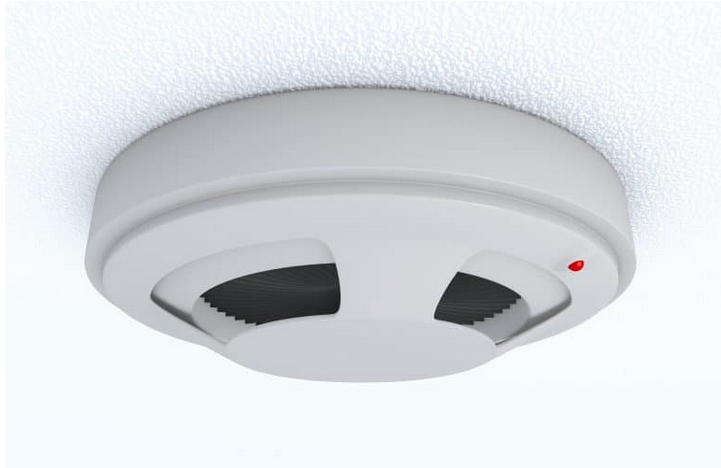
\includegraphics[width=0.5\textwidth]{Imagenes/Introduccion/Intro_ejemplo.png}}
        \caption{Epígrafe de prueba en Intro.}
        \label{fig:IntroImage}
    \end{figure}

    \section{Marco Teórico}
    Aquí se ejemplifica el Marco Teórico. También se referencia la Figura~\ref{fig:IntroImage},
    la cual pertenece a la Introducción.
    
    \begin{figure}[ht]
      \centering
      \frame{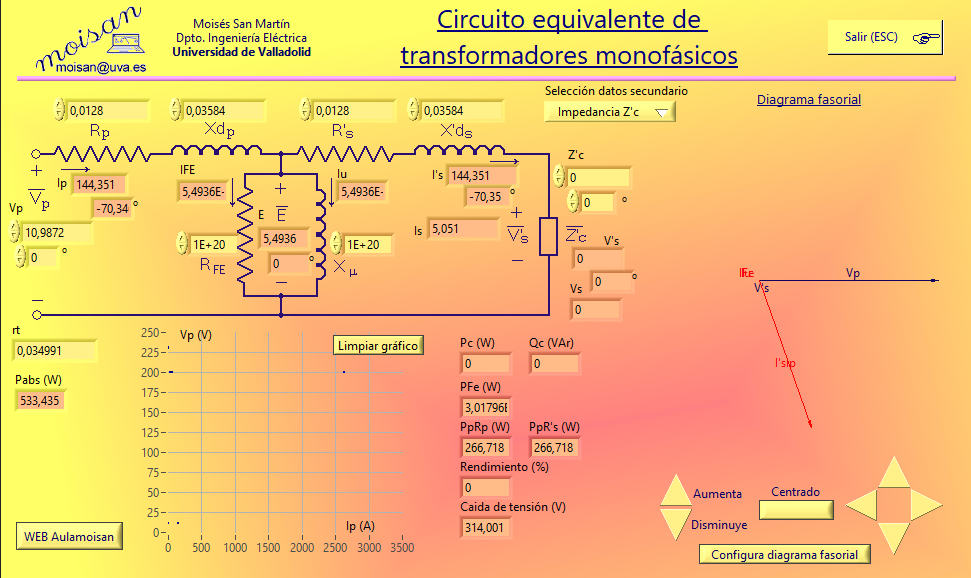
\includegraphics[width=\textwidth]{Imagenes/MarcoTeorico/MarcTeo_ejemplo.png}}
      \caption{Epígrafe de ejemplo del Marco Teórico.}
      \label{fig:MarcTeoImage}
  \end{figure}


    \section{Actividad Práctica}

  En esta sección iría la consigna.

      \begin{figure}[ht]
      \centering
      \frame{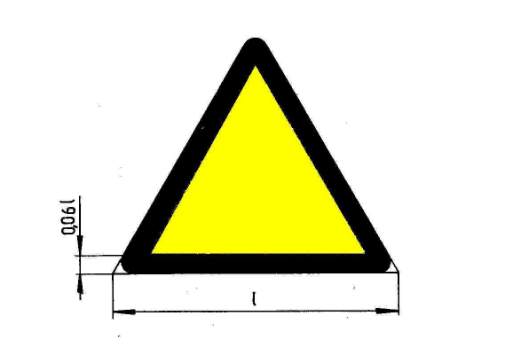
\includegraphics[width=\textwidth]{Imagenes/ActividadPractica/ActPra_ejemplo.png}}
      \caption{Epígrafe de ejemplo de Actividad Práctica.}
      \label{fig:ActPraImage}
  \end{figure}


    \subsection{Subsección 1}

    \subsection{Subsección 2}

    \subsection{Subsección 3}

    \subsection{Subsección 4}

    \subsection{Subsección 5}


    \section{Conclusiones}

  A modo de ejemplo, referencio las imágenes de las secciones. Estas corresponden a las Figuras \ref{fig:IntroImage}, \ref{fig:MarcTeoImage} y \ref{fig:ActPraImage}.

   \begin{figure}[ht]
      \centering
      \frame{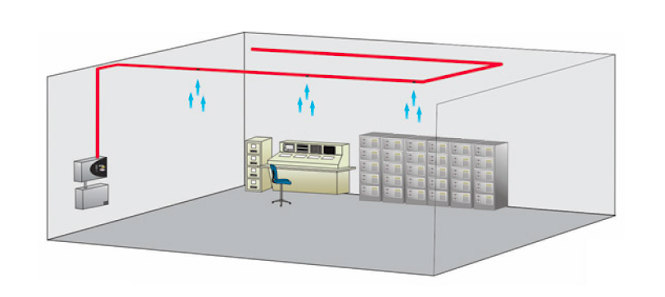
\includegraphics[width=\textwidth]{Imagenes/Conclusiones/Concl_ejemplo.png}}
      \caption{Epígrafe de ejemplo de la Conclusión.}
      \label{fig:ConclImage}
  \end{figure}


  
\end{document}
